\subsection{General Use-Case Diagram}
\noindent Placeholder for diagram:
\begin{center}
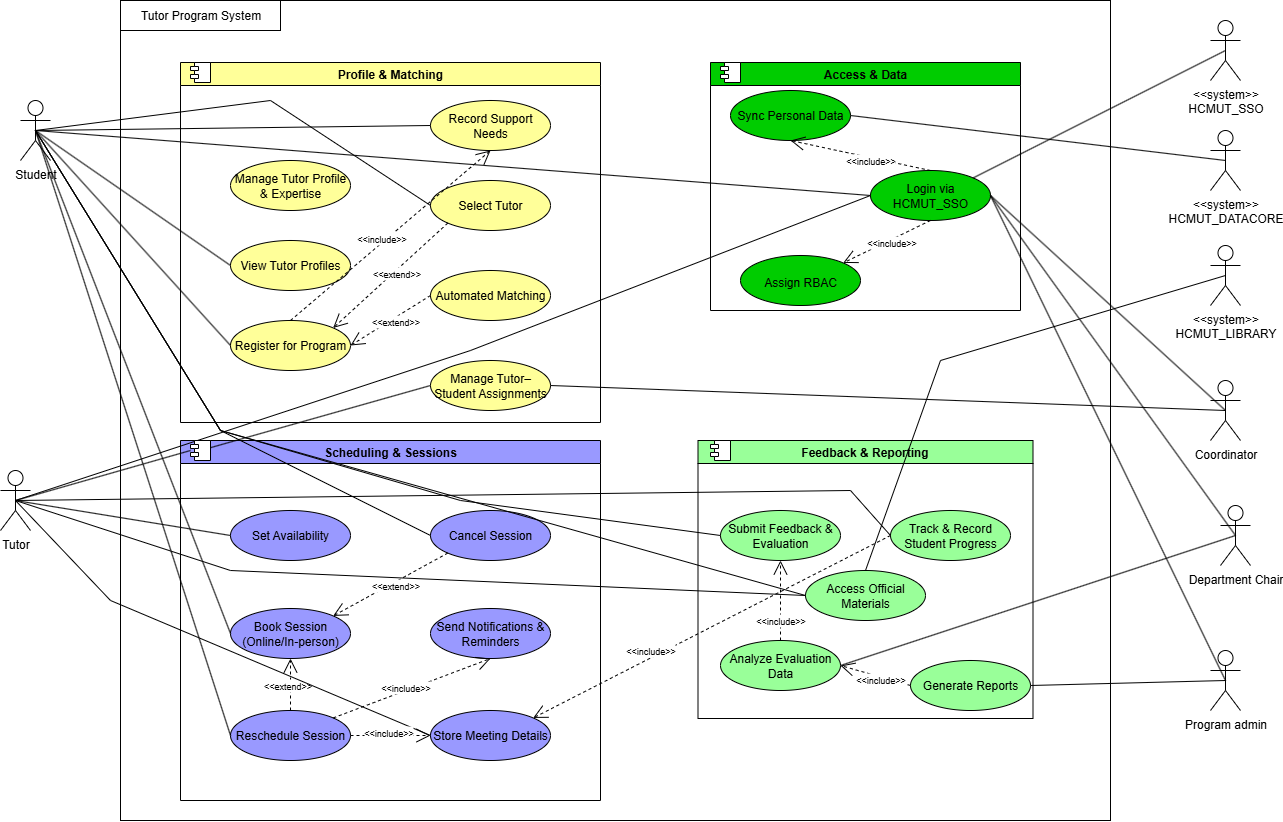
\includegraphics[width=0.9\linewidth]{images/usecase-general.png}
\end{center}

\begin{center}
\textbf{Figure 1:} General Tutor program system
\end{center}
\clearpage
\subsection{UC-01 Log in \& Profile Management}
\begin{center}
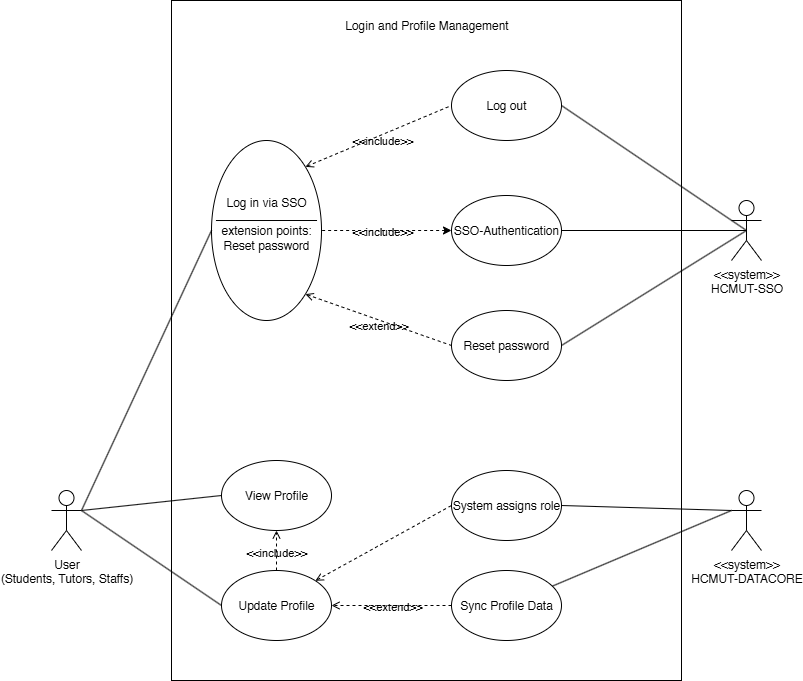
\includegraphics[width=0.9\linewidth]{images/UC-01.png}
\end{center}

\begin{center}
\textbf{Figure 2:}  Log in and Manage Profile
\end{center}  


\begin{table}[h!]
\centering
\begin{tabular}{|p{3cm}|p{11cm}|}
\hline
\textbf{Use-case ID} & UC-01a \\
\hline
\textbf{Use-case name} & Login via SSO \\
\hline
\textbf{Use-case overview} & To allow students, tutors, and staff to log in securely via HCMUT\_SSO with role assignment handled by the system. \\
\hline
\textbf{Actors} & User (Students, Tutors, Staff), HCMUT\_SSO, System \\
\hline
\textbf{Preconditions} & 
1. User has valid SSO credentials. \newline
2. HCMUT\_SSO service is available. \\
\hline
\textbf{Trigger} & User selects the ``Login via SSO'' option. \\
\hline
\textbf{Steps} & 
1. User initiates login via HCMUT\_SSO. \newline
2. System sends authentication request to SSO service. \newline
3. HCMUT\_SSO validates credentials. \newline
4. On success, the system fetches user data and assigns role. \newline
5. On failure, the system denies access. \\
\hline
\textbf{Postconditions} & User is authenticated and session established; role assignment is ready for system use. \\
\hline
\textbf{Alternative Flows} & 
A1: Invalid login → Access denied with error message. \newline
A2: Role update in DATACORE synced during login. \\
\hline
\textbf{Exception Flow} & 
1. SSO service unavailable → System shows maintenance/unavailable message. \newline
2. Network error → User prompted to retry login. \\
\hline
\end{tabular}
\caption{Use Case UC-01a: Login via SSO}
\end{table}


\begin{table}[h!]
\centering
\begin{tabular}{|p{3cm}|p{11cm}|}
\hline
\textbf{Use-case ID} & UC-01b \\
\hline
\textbf{Use-case name} & Profile Management \\
\hline
\textbf{Use-case overview} & To allow students and tutors to view and update their profiles, with core data synchronized from HCMUT\_DATACORE. \\
\hline
\textbf{Actors} & Student, Tutor, HCMUT\_DATACORE, System \\
\hline
\textbf{Preconditions} & 
1. User is authenticated via SSO. \newline
2. Profile data exists in DATACORE. \\
\hline
\textbf{Trigger} & User selects the ``View/Update Profile'' option. \\
\hline
\textbf{Steps} & 
1. System retrieves profile information from DATACORE. \newline
2. User views profile fields (ID, name, email, faculty, role). \newline
3. User updates non-core profile details. \newline
4. System validates and saves changes. \newline
5. System syncs updated data with DATACORE. \\
\hline
\textbf{Postconditions} & User profile is updated and synchronized with DATACORE; changes are timestamped and logged. \\
\hline
\textbf{Alternative Flows} & 
A1: DATACORE unavailable → Updates stored locally until sync resumes. \\
\hline
\textbf{Exception Flow} & 
1. Invalid update request → System rejects and shows error. \newline
2. Sync conflict with DATACORE → DATACORE treated as source of truth. \\
\hline
\end{tabular}
\caption{Use Case UC-01b: Profile Management}
\end{table}


\clearpage
\subsection{UC-02 Tutor--Student Matching}


\begin{center}
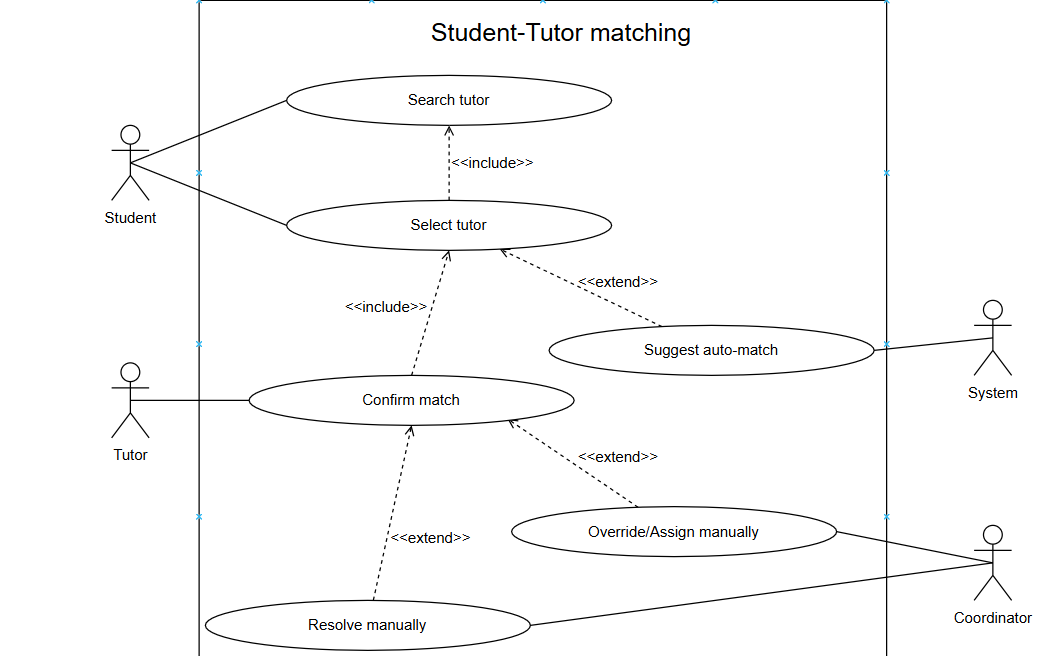
\includegraphics[width=0.9\linewidth]{images/UC-02.png}
\end{center}

\begin{center}
\textbf{Figure 3:}  Tutor--Student Matching
\end{center}

\begin{table}[h!]
\centering
\begin{tabular}{|p{3cm}|p{11cm}|}
\hline
\textbf{Use-case ID} & UC-02 \\
\hline
\textbf{Use-case name} & Tutor--Student Matching \\
\hline
\textbf{Use-case overview} & To allow students to search and select tutors manually or request an automated match, with tutor confirmation and coordinator intervention when necessary. \\
\hline
\textbf{Actors} & Student (primary), Tutor, Coordinator, System \\
\hline
\textbf{Preconditions} & 
1. Student and tutor profiles exist in the system. \newline
2. The system is operational and accessible. \newline
3. Student is authenticated in the system. \\
\hline
\textbf{Trigger} & Student initiates a search for tutors or requests an auto-match. \\
\hline
\textbf{Steps} &
1. Student searches for tutors by subject, availability, or preferences. \newline
2. Student selects a tutor; a pending match is created. \newline
3. System may suggest an auto-match (ranked list) based on the student's criteria. \newline
4. Tutor reviews the pending match and confirms the match. \newline
5. If confirmed, the system finalizes and logs the pairing. \\
\hline
\textbf{Postconditions} & A tutor--student pairing is established and logged in the system. \\
\hline
\textbf{Alternative Flows} & 
1. Auto-match rejected by student or tutor → Coordinator resolves manually. \newline
2. No tutors found → System suggests broadening search criteria. \newline
3. Tutor does not respond within time limit → Coordinator is notified to assign a tutor. \\
\hline
\textbf{Exception Flow} & 
1. Network failure prevents search or confirmation (system prompts user to retry). \newline
2. Tutor or student profile missing/corrupted → System logs an error and notifies Coordinator. \\
\hline
\end{tabular}
\caption{Use Case UC-02: Tutor--Student Matching}
\end{table}

\clearpage
 \subsection{UC-03 Session Scheduling Management}


\begin{center}
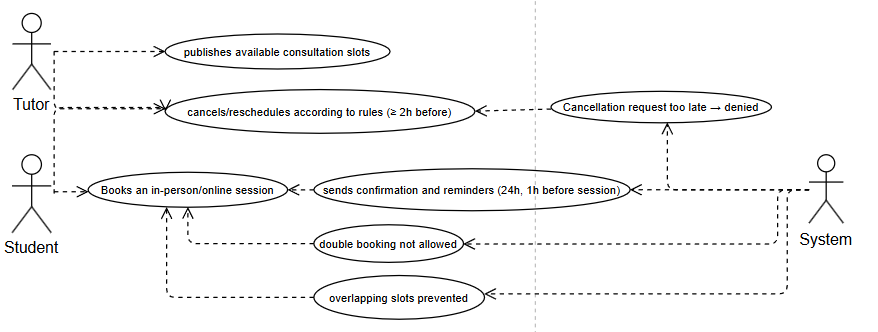
\includegraphics[width=0.9\linewidth]{images/UC-03.png}
\end{center}

\begin{center}
\textbf{Figure 4:}  Session Scheduling Management
\end{center}

\begin{table}[h!]
\centering
\begin{tabular}{|p{3cm}|p{11cm}|}
\hline
\textbf{Use-case ID} & UC-03 \\
\hline
\textbf{Use-case name} & Session Scheduling Management \\
\hline
\textbf{Use-case overview} & This use case describes the end-to-end process of session scheduling between a student and a tutor, including slot publication, booking, cancellation, rescheduling, and automatic notifications. \\
\hline
\textbf{Actors} & Student, Tutor, System \\
\hline
\textbf{Preconditions} & 
1. Student is matched with a tutor. \newline
2. Tutor has published available slots. \newline
3. System is operational and connected to the scheduling database. \\
\hline
\textbf{Trigger} & 
1. Tutor publishes or edits availability slots. \newline
2. Student attempts to book a session. \newline
3. Student or tutor submits a cancellation or rescheduling request. \\
\hline
\textbf{Steps} & 
1. Tutor publishes available consultation slots. \newline
2. System prevents overlapping slots. \newline
3. Student views available slots. \newline
4. If a slot is suitable, student books a session. \newline
5. System prevents double-booking and stores session details. \newline
6. System confirms the booking and sends notifications. \newline
7. Before the session, the system sends reminders (24h and 1h before). \newline
8. Student or tutor may request cancellation or rescheduling at least 2 hours before the session. \newline
9. System validates the request: if valid, cancels/reschedules and sends notifications; otherwise denies the request. \\
\hline
\textbf{Postconditions} & 
1. Session is successfully scheduled, rescheduled, or cancelled according to rules. \newline
2. Notifications and reminders are delivered to all relevant parties. \\
\hline
\textbf{Exception Flow} & 
1. Overlapping slots → publishing is denied. \newline
2. Double-booking attempt → booking is denied. \newline
3. No suitable slot → student is prompted to wait or check later. \newline
4. Late cancellation → request is denied. \\
\hline
\end{tabular}
\caption{Use Case UC-03: Session Scheduling Management}
\end{table}

\clearpage
\subsection{UC-04 Feedback \& Progress Tracking}
\begin{center}
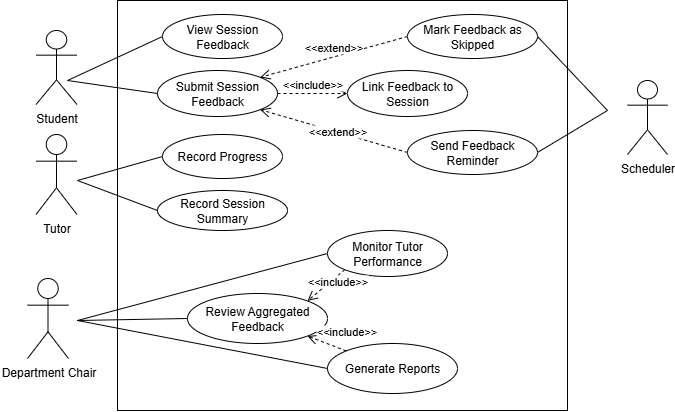
\includegraphics[width=0.9\linewidth]{images/UC-04.png}
\end{center}

\begin{center}
\textbf{Figure 5:}  Submit Session Feedback
\end{center}


\begin{center}
\begin{longtable}{|p{3cm}|p{11cm}|}
\hline
\textbf{Use-case ID} & UC-04a \\ 
\hline
\textbf{Use-case name} & Submit Session Feedback \\ 
\hline
\textbf{Use-case overview} & To allow a student to submit structured feedback after a tutoring session. The feedback is linked to the session and stored for later evaluation and reporting. \\ 
\hline
\textbf{Actors} & 
\begin{itemize}
    \item Student (primary)
    \item Scheduler (secondary, for reminders and marking ‘Skipped’)
\end{itemize} \\ 
\hline
\textbf{Preconditions} & 
\begin{enumerate}
    \item A tutoring session has been completed.
    \item The system is running and accessible.
    \item Student is authenticated in the system.
\end{enumerate} \\ 
\hline
\textbf{Trigger} & The student clicks the ``Submit Feedback'' option after the session is completed. \\ 
\hline
\textbf{Main Flow (Steps)} & 
\begin{enumerate}
    \item System displays a feedback form linked to the completed session.
    \item Student fills in and submits the structured feedback.
    \item System validates the input and saves the feedback in the database.
    \item System links the feedback to the corresponding session.
\end{enumerate} \\ 
\hline
\textbf{Postconditions} & 
\begin{itemize}
    \item Feedback is stored in the database and linked to the correct session.
    \item If skipped, the system records a ``Feedback Skipped'' status for that session.
    \item Data is available for tutors and department chairs in aggregated reports.
\end{itemize} \\ 
\hline
\textbf{Alternative Flows} & 
\begin{enumerate}
    \item \textbf{Multiple Session Feedback:} If multiple sessions are pending, the system displays a list and allows the student to submit feedback sequentially.
    \item \textbf{Draft Save/Connection Loss:} The student may save incomplete feedback as a draft and return later. System automatically saves the draft if connection is lost before final submission.
    \item \textbf{Feedback Revision:} Within a defined grace period (e.g., 24h), the student may edit and resubmit feedback; the updated version replaces the original.
    \item \textbf{Skipped Feedback:} If no feedback is submitted within the allowed time, the Scheduler triggers a process to mark the session's feedback status as ``Skipped.'' 
\end{enumerate} \\ 
\hline
\textbf{Exception Flows} & 
\begin{itemize}
    \item \textbf{Database Error:} If the system fails to save the final submission due to a database error, it logs the error and prompts the student to retry later.
    \item \textbf{Missing Session Record:} If the session record is missing or corrupted, the system logs an error and notifies the coordinator.
\end{itemize} \\ 
\hline
\caption{Use Case UC-04a: Submit Session Feedback}
\end{longtable}
\end{center}

\begin{center}
\begin{longtable}{|p{3cm}|p{11cm}|}
\hline
\textbf{Use-case ID} & UC-04b \\
\hline
\textbf{Use-case name} & Record Student Progress \\
\hline
\textbf{Use-case overview} & To allow tutors to record student progress and optionally add session summaries for reference and tracking purposes. \\
\hline
\textbf{Actors} & Tutor \\
\hline
\textbf{Preconditions} & 
1. A tutoring session has been completed. \newline
2. The system is running and accessible. \newline
3. Tutor is authenticated in the system. \\
\hline
\textbf{Trigger} & Tutor accesses the session record and selects “Record Progress.” \\
\hline
\textbf{Steps} & 
1. Tutor opens the specific session record. \newline
2. Tutor enters progress notes and, optionally, a session summary. \newline
3. Tutor submits the record. \newline
4. System validates the input and saves the record, linking it to the session. \\
\hline
\textbf{Postconditions} & 
1. Student progress and optional session summary are saved. \newline
2. Data is linked to the session and available for departmental review. \\
\hline
\textbf{Alternative Flows} & 
A1: Optional Summary → Tutor skips writing a session summary (only progress notes are saved). \newline
A2: Draft Save / Connection Loss → Tutor may save incomplete notes as a draft; the system auto-saves the draft if the connection is lost. \newline
A3: Note Revision → Within a 24-hour grace period, tutor may edit and resubmit notes; the new version replaces the previous record. \\
\hline
\textbf{Exception Flow} & 
1. Database error → System logs the issue and notifies the tutor to retry. \newline
2. Missing or locked session → System notifies the tutor and logs the error. \\
\hline
\textbf{Priority} & Should \\
\hline
\caption{Use Case UC-04b: Record Student Progress}
\end{longtable}
\end{center}

\begin{center}
\begin{longtable}{|p{3cm}|p{11cm}|}
\hline
\textbf{Use-case ID} & UC-04c \\ 
\hline
\textbf{Use-case name} & Review Aggregated Reports (Feedback \& Progress) \\ 
\hline
\textbf{Overview} & To allow the department chair to review aggregated feedback and progress data for monitoring tutor performance and program effectiveness. \\ 
\hline
\textbf{Actors} & Department Chair \\ 
\hline
\textbf{Preconditions} & 
\begin{enumerate}
    \item Feedback and progress records exist in the database.
    \item The system is running and accessible.
    \item Department Chair is authenticated in the system.
\end{enumerate} \\ 
\hline
\textbf{Trigger} & Department Chair selects ``Aggregated Reports Overview.'' \\ 
\hline
\textbf{Main Flow (Steps)} & 
\begin{enumerate}
    \item Department Chair selects report criteria (e.g., date range, tutor, course).
    \item System retrieves all relevant feedback and progress data.
    \item System processes and displays aggregated statistics, charts, or reports.
\end{enumerate} \\ 
\hline
\textbf{Postconditions} & 
\begin{itemize}
    \item Aggregated data is available for decision-making.
    \item Reports may be exported or stored for institutional use.
\end{itemize} \\ 
\hline
\textbf{Alternative Flows} & 
\begin{itemize}
    \item[AF1] \textbf{Filtering:} Department Chair filters or drills down data by tutor, course, or specific time period.
    \item[AF2] \textbf{Export Report:} Department Chair exports the report in a chosen format (e.g., PDF, CSV) for external analysis.
\end{itemize} \\ 
\hline
\textbf{Exception Flows} & 
\begin{itemize}
    \item \textbf{Database/Retrieval Failure:} If database retrieval fails, the system shows a technical error message and logs the issue for system administrators.
    \item \textbf{No Data:} If no data matches the selected criteria, the system displays a clear message: ``No data available for this selection.''
\end{itemize} \\ 
\hline
\caption{Use Case UC-04c: Review Aggregated Reports}
\end{longtable}
\end{center}




% \begin{center}
% 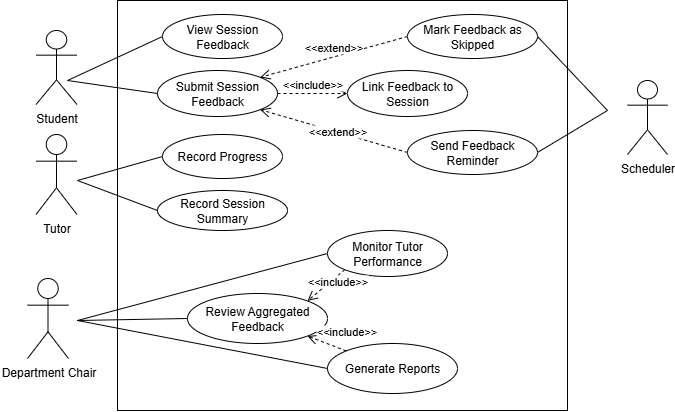
\includegraphics[width=0.9\linewidth]{images/UC-04.png}
% \end{center}

% \begin{center}
% \textbf{Figure 5:}  Submit Session Feedback
% \end{center}


% \begin{table}[h!]
% \centering
% \begin{tabular}{|p{3cm}|p{11cm}|}
% \hline
% \textbf{Use-case ID} & UC-04 \\
% \hline
% \textbf{Use-case name} & Submit Session Feedback \\
% \hline
% \textbf{Use-case overview} & To allow a student to submit structured feedback after a tutoring session. The feedback is linked to the session and stored for later evaluation and reporting. \\
% \hline
% \textbf{Actors} & Student (primary), Scheduler (secondary, for reminders) \\
% \hline
% \textbf{Preconditions} & 
% 1. A tutoring session has been completed. \newline
% 2. The system is running and accessible. \newline
% 3. Student is authenticated in the system. \\
% \hline
% \textbf{Trigger} & The student clicks the ``Submit Feedback'' option after the session is completed. \\
% \hline
% \textbf{Steps} & 
% 1. System displays a feedback form linked to the completed session. \newline
% 2. Student fills in and submits the structured feedback. \newline
% 3. System validates the input and saves the feedback in the database. \newline
% 4. System links the feedback to the corresponding session. \newline
% 5. If no feedback is submitted within the allowed time, the Scheduler triggers reminders. \newline
% 6. If the deadline passes without submission, the system marks the feedback as ``Skipped.'' \\
% \hline
% \textbf{Postconditions} & 
% 1. Feedback is stored in the database and linked to the correct session. \newline
% 2. If skipped, the system records a ``Feedback Skipped'' status for that session. \newline
% 3. Data is available for tutors and department chairs in aggregated reports. \\
% \hline
% \textbf{Alternative Flows} & 
% 1. Multiple Session Feedback → If multiple sessions are pending, the system displays a list and allows the student to submit feedback sequentially. \newline
% 2. Draft Save → The student may save incomplete feedback as a draft and return later within the allowed timeframe. \newline
% 3. Feedback Revision → Within 24h, the student may edit and resubmit feedback; the updated version replaces the original record. \\
% \hline
% \textbf{Exception Flow} & 
% 1. If the student loses connection before submission, the system prompts the student to retry. \newline
% 2. If the session record is missing or corrupted, the system logs an error and notifies the coordinator. \\
% \hline
% \end{tabular}
% \caption{Use Case UC-04: Submit Session Feedback}
% \end{table}
\clearpage
\subsection{UC-05 Reporting \& Analytics}
\begin{center}
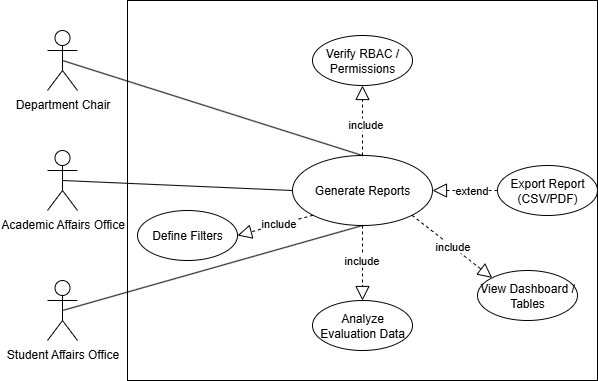
\includegraphics[width=0.9\linewidth]{images/UC-05.png}
\end{center}

\begin{center}
\textbf{Figure 6:}  Reporting and Analytics
\end{center}


\begin{table}[h!]
\centering
\begin{tabular}{|p{3cm}|p{11cm}|}
\hline
\textbf{Use-case ID} & UC-05a \\
\hline
\textbf{Use-case name} & Generate Departmental Report \\
\hline
\textbf{Use-case overview} & Department Chair generates a department-level report (attendance, performance, session counts) for academic monitoring and decisions. \\
\hline
\textbf{Actors} & Department Chair \\
\hline
\textbf{Preconditions} & 
1. Authenticated and authorized to view departmental reports. \newline
2. Sessions, feedback, and (if applicable) progress data exist. \newline
3. System is operational. \\
\hline
\textbf{Trigger} & Chair opens ``Reporting'' and selects ``Departmental Report''. \\
\hline
\textbf{Steps} & 
1. Set filters (term/date, program/department, tutor/cohort). \newline
2. System retrieves and analyzes metrics (attendance, performance, session counts). \newline
3. System displays tables/charts with data-source notes. \newline
4. Optional: Export CSV/PDF with metadata (generation time, filters, version); log action. \\
\hline
\textbf{Postconditions} & 
1. Departmental report displayed; optional file generated. \newline
2. Action recorded in the audit log. \\
\hline
\textbf{Alternative Flows} & 
1. Change filters/scope $\rightarrow$ system refreshes results. \\
\hline
\textbf{Exception Flow} & 
1. No data for selected criteria $\rightarrow$ show ``No data available for this selection.'' \newline
2. Export error (I/O or size) $\rightarrow$ suggest narrowing scope or retrying. \newline
3. Data source unavailable $\rightarrow$ show service notice; allow retry when available. \\
\hline
\end{tabular}
\caption{Use Case UC-05a: Generate Departmental Report}
\end{table}

\begin{table}[h!]
\centering
\begin{tabular}{|p{3cm}|p{11cm}|}
\hline
\textbf{Use-case ID} & UC-05b \\
\hline
\textbf{Use-case name} & View Tutor Workload Dashboard \\
\hline
\textbf{Use-case overview} & Academic Affairs views tutor workload and student demand to allocate resources effectively. \\
\hline
\textbf{Actors} & Academic Affairs Office \\
\hline
\textbf{Preconditions} & 
1. Authenticated and authorized for workload dashboards. \newline
2. Sessions/booking and feedback data exist. \newline
3. System is operational. \\
\hline
\textbf{Trigger} & Office opens ``Workload \& Demand'' dashboard. \\
\hline
\textbf{Steps} & 
1. Select filters (term/date, department/program). \newline
2. System aggregates tutor load and demand indicators. \newline
3. System displays dashboard (tables/charts, drill-down). \newline
4. Optional: Export CSV/PDF with metadata; log action. \\
\hline
\textbf{Postconditions} & 
1. Workload dashboard visible; optional export ready. \newline
2. Access recorded in the audit log. \\
\hline
\textbf{Alternative Flows} & 
1. Drill-down by tutor/program $\rightarrow$ refresh view. \\
\hline
\textbf{Exception Flow} & 
1. No data for selected criteria $\rightarrow$ show ``No data available for this selection.'' \newline
2. Export error (I/O or size) $\rightarrow$ suggest narrowing scope or retrying. \newline
3. Data source unavailable $\rightarrow$ show service notice; allow retry when available. \\
\hline
\end{tabular}
\caption{Use Case UC-05b: View Tutor Workload Dashboard}
\end{table}

\begin{table}[h!]
\centering
\begin{tabular}{|p{3cm}|p{11cm}|}
\hline
\textbf{Use-case ID} & UC-05c \\
\hline
\textbf{Use-case name} & Generate Participation Report \\
\hline
\textbf{Use-case overview} & Student Affairs generates participation reports for credit/scholarship consideration. \\
\hline
\textbf{Actors} & Student Affairs Office \\
\hline
\textbf{Preconditions} & 
1. Authenticated and authorized for participation reports. \newline
2. Sessions and attendance/feedback records exist. \newline
3. System is operational. \\
\hline
\textbf{Trigger} & Office selects ``Participation Report''. \\
\hline
\textbf{Steps} & 
1. Choose filters (term/date, cohort, program, thresholds). \newline
2. System compiles participation metrics and eligibility indicators. \newline
3. System displays results; Optional: export CSV/PDF with metadata; log action. \\
\hline
\textbf{Postconditions} & 
1. Participation report displayed; optional file generated. \newline
2. Action logged. \\
\hline
\textbf{Alternative Flows} & 
1. Adjust filters/criteria $\rightarrow$ refresh results. \\
\hline
\textbf{Exception Flow} & 
1. No data for selected criteria $\rightarrow$ show ``No data available for this selection.'' \newline
2. Export error (I/O or size) $\rightarrow$ suggest narrowing scope or retrying. \newline
3. Data source unavailable $\rightarrow$ show service notice; allow retry when available. \\
\hline
\end{tabular}
\caption{Use Case UC-05c: Generate Participation Report}
\end{table}

\clearpage
\subsection{UC-06 Integration with HCMUT Infrastructure}

\begin{center}
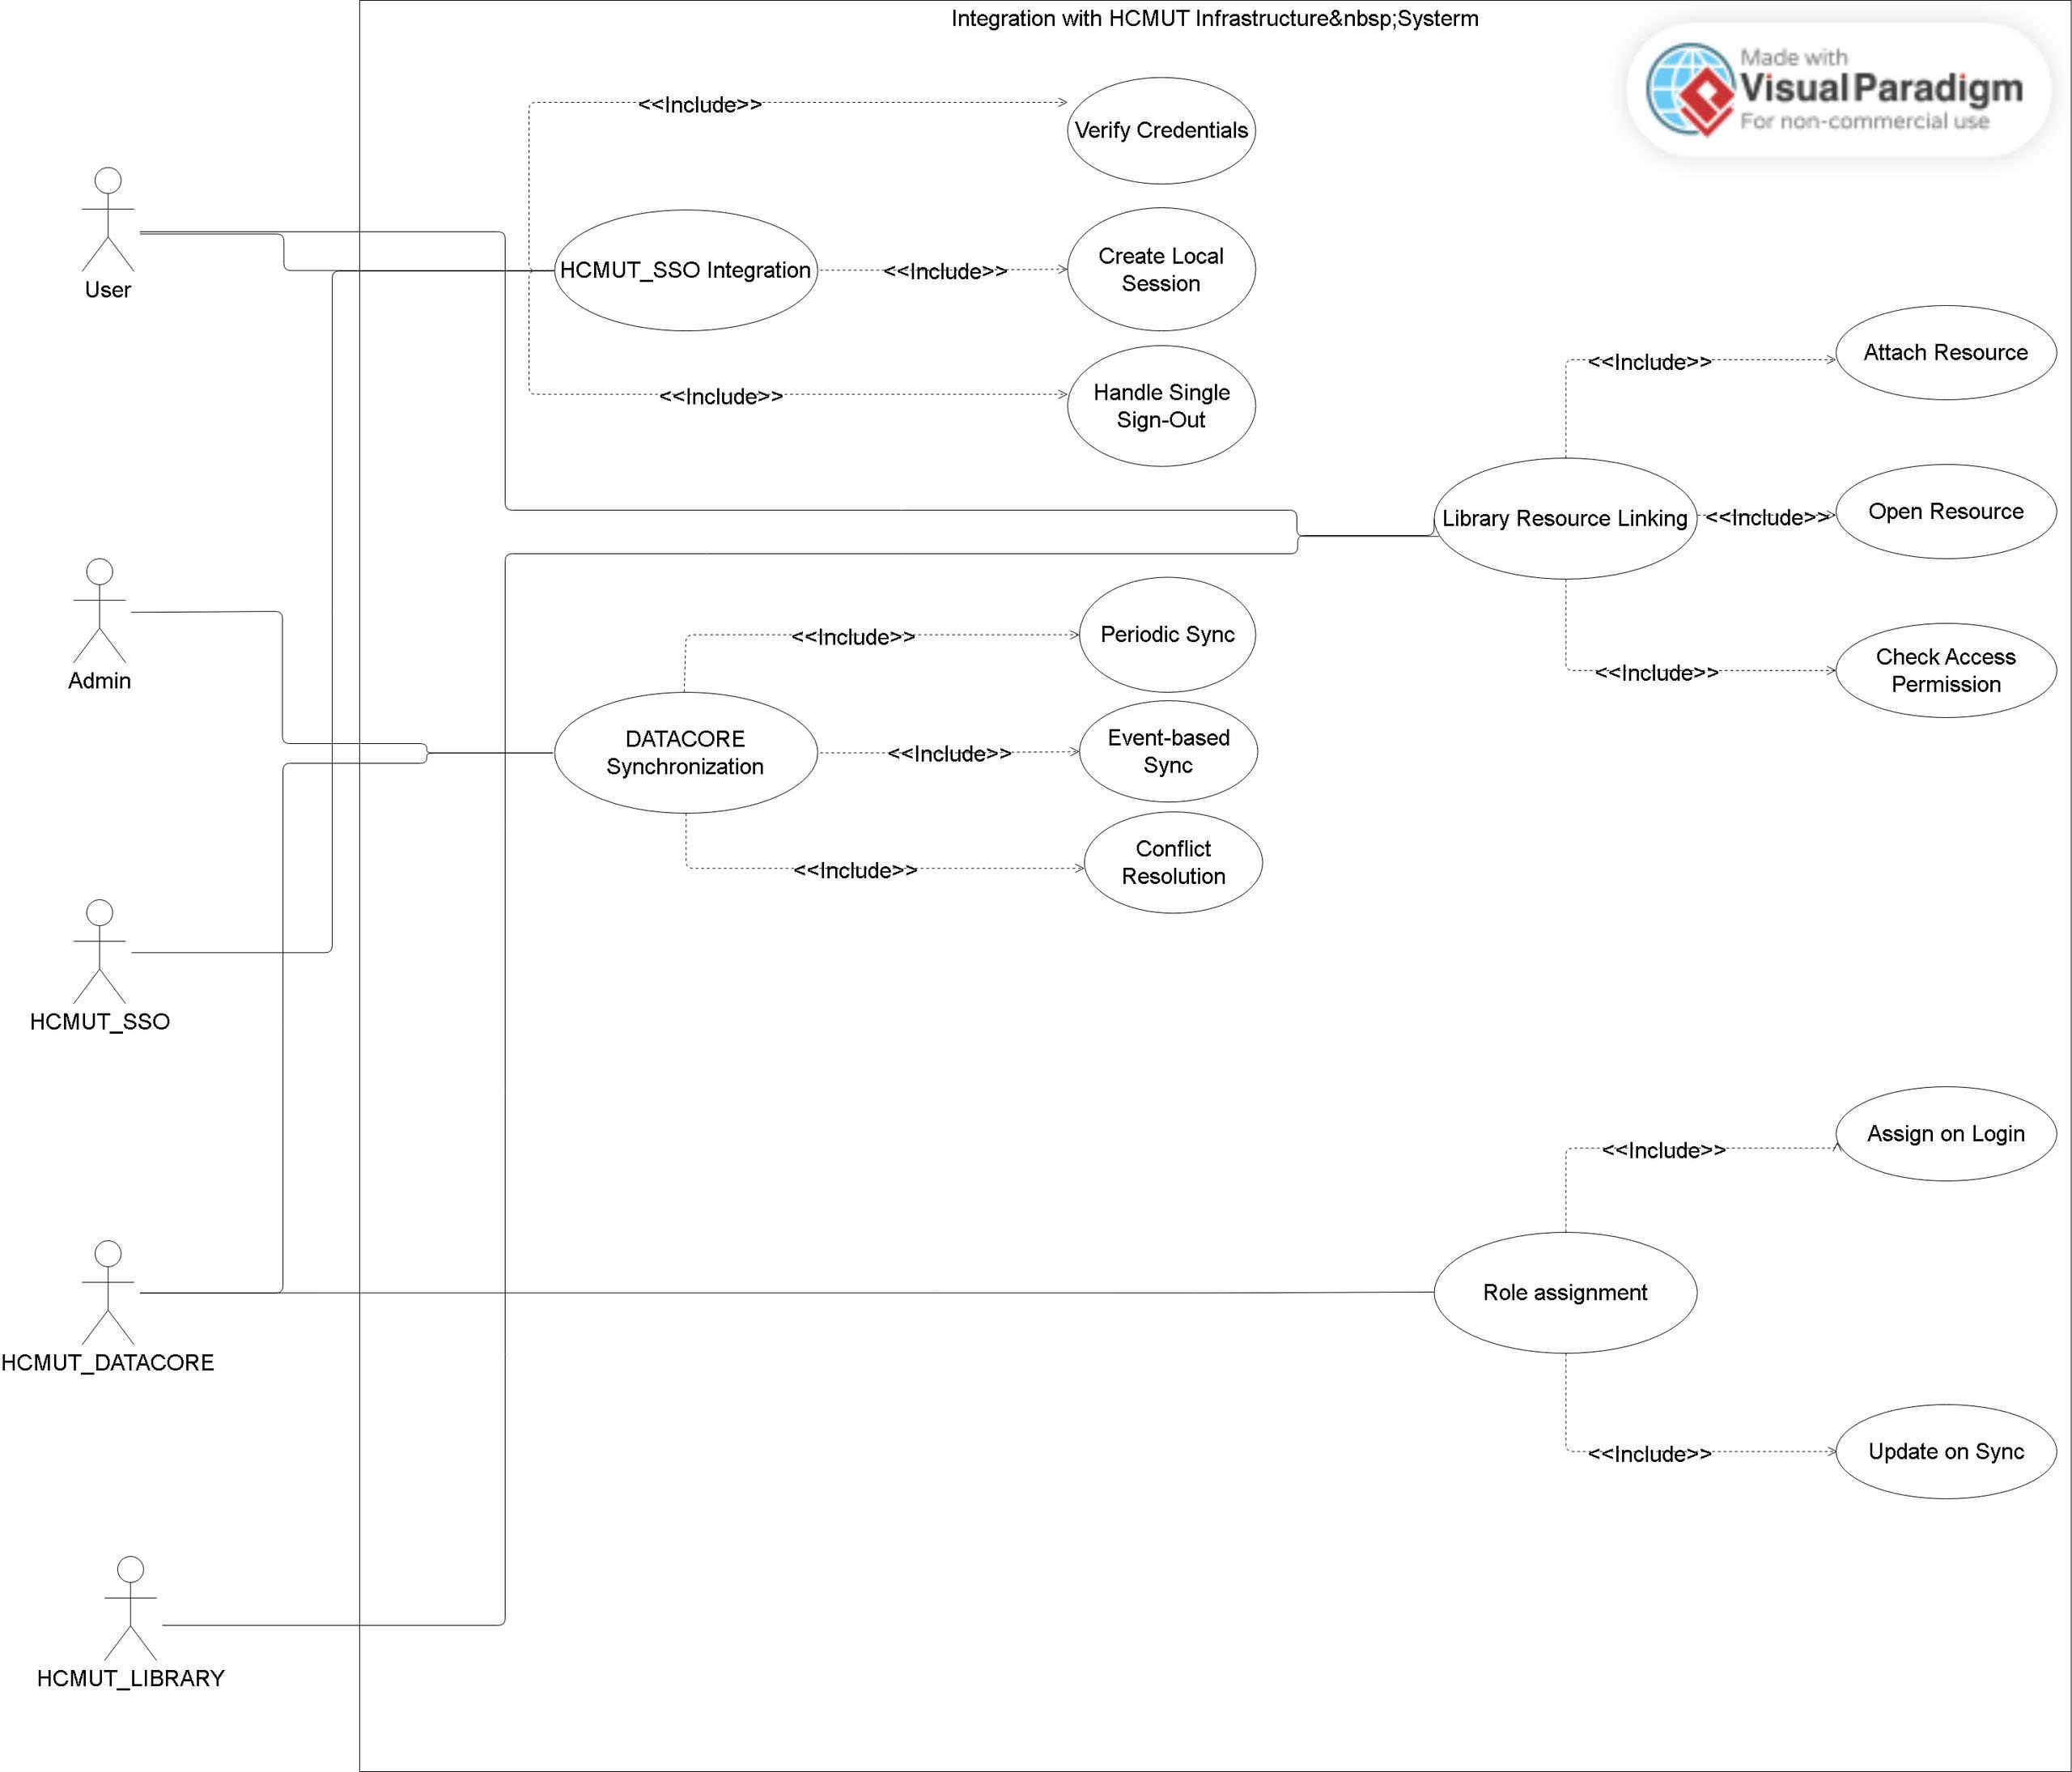
\includegraphics[width=0.9\linewidth]{images/UC-06.png}
\end{center}

\begin{center}
\textbf{Figure 7:}  Integration with HCMUT Infrastructure
\end{center}

\begin{table}[h!]
\centering
\begin{tabular}{|p{3cm}|p{11cm}|}
\hline
\textbf{Use-case ID} & UC-06.01 \\
\hline
\textbf{Use-case name} & HCMUT\_SSO Integration \\
\hline
\textbf{Use-case overview} & The system integrates with HCMUT\_SSO for unified authentication, allowing users to log in using university credentials and automatically manage single sign-out. \\
\hline
\textbf{Actors} & User, System, HCMUT\_SSO \\
\hline
\textbf{Preconditions} & HCMUT\_SSO service is operational and reachable. \\
\hline
\textbf{Trigger} & User initiates login via HCMUT\_SSO. \\
\hline
\textbf{Steps} & 
1. User selects “Login with HCMUT\_SSO”. \newline
2. System redirects to the authentication portal. \newline
3. HCMUT\_SSO validates credentials and returns a token. \newline
4. System verifies the token and creates a session. \newline
5. Upon sign-out at SSO, the system terminates the local session. \\
\hline
\textbf{Postconditions} & 
1. User is successfully authenticated. \newline
2. Single sign-out ensures session consistency. \\
\hline
\textbf{Exception Flow} & 
1. Invalid or expired token → login attempt rejected. \newline
2. SSO service unavailable → system displays maintenance message. \\
\hline
\textbf{Priority} & Must \\
\hline
\end{tabular}
\caption{Use Case UC-06.01: HCMUT\_SSO Integration}
\end{table}


\begin{table}[h!]
\centering
\begin{tabular}{|p{3cm}|p{11cm}|}
\hline
\textbf{Use-case ID} & UC-06.02 \\
\hline
\textbf{Use-case name} & DATACORE Synchronization \\
\hline
\textbf{Use-case overview} & The system synchronizes personal and academic data from HCMUT\_DATACORE periodically or in near real-time to ensure data consistency and reduce manual entry. \\
\hline
\textbf{Actors} & System, HCMUT\_DATACORE, Administrator \\
\hline
\textbf{Preconditions} & DATACORE APIs are online and accessible. \\
\hline
\textbf{Trigger} & Scheduled synchronization or data-change event detected. \\
\hline
\textbf{Steps} & 
1. System triggers synchronization with DATACORE. \newline
2. Retrieve updated profiles and academic data. \newline
3. Validate and compare data with local records. \newline
4. Update local data using DATACORE as source of truth. \newline
5. Log synchronization status and timestamp. \\
\hline
\textbf{Postconditions} & 
1. Local data mirrors DATACORE. \newline
2. Synchronization events logged for auditing. \\
\hline
\textbf{Exception Flow} & 
1. Connection timeout or API error → retry with exponential backoff. \newline
2. Invalid data format → skip record and log validation error. \\
\hline
\textbf{Priority} & Must \\
\hline
\end{tabular}
\caption{Use Case UC-06.02: DATACORE Synchronization}
\end{table}

\begin{table}[h!]
\centering
\begin{tabular}{|p{3cm}|p{11cm}|}
\hline
\textbf{Use-case ID} & UC-06.03 \\
\hline
\textbf{Use-case name} & Role Assignment \\
\hline
\textbf{Use-case overview} & The system automatically assigns user roles (student, tutor, coordinator, department chair, or administrator) based on centralized role data from DATACORE and SSO. \\
\hline
\textbf{Actors} & User, System, HCMUT\_DATACORE \\
\hline
\textbf{Preconditions} & User is authenticated via SSO and DATACORE role data is available. \\
\hline
\textbf{Trigger} & User login or scheduled role update. \\
\hline
\textbf{Steps} & 
1. Retrieve role mapping from DATACORE. \newline
2. Match user ID with centralized role data. \newline
3. Assign permissions based on role. \newline
4. Apply changes in access-control policies. \newline
5. Log the role-assignment event. \\
\hline
\textbf{Postconditions} & 
1. User roles align with centralized data. \newline
2. Updated permissions take effect immediately. \\
\hline
\textbf{Exception Flow} & 
1. Role data missing → assign default “student” role and notify admin. \newline
2. Role conflict → logged and flagged for manual verification. \\
\hline
\textbf{Priority} & Must \\
\hline
\end{tabular}
\caption{Use Case UC-06.03: Role Assignment}
\end{table}


\begin{table}[h!]
\centering
\begin{tabular}{|p{3cm}|p{11cm}|}
\hline
\textbf{Use-case ID} & UC-06.04 \\
\hline
\textbf{Use-case name} & Library Resource Linking \\
\hline
\textbf{Use-case overview} & The system connects with HCMUT\_LIBRARY to let tutors and students attach or access library materials securely within tutoring sessions or summaries. \\
\hline
\textbf{Actors} & Student, Tutor, System, HCMUT\_LIBRARY \\
\hline
\textbf{Preconditions} & Library API and authentication services are available. \\
\hline
\textbf{Trigger} & User attaches or opens a library resource. \\
\hline
\textbf{Steps} & 
1. User searches or selects a library resource. \newline
2. System requests metadata and access permissions. \newline
3. Verify user eligibility via role-based access. \newline
4. Attach or open the resource in session view. \newline
5. Log the access event. \\
\hline
\textbf{Postconditions} & 
1. Resource successfully linked to the session or summary. \newline
2. Access rights enforced per library policy. \\
\hline
\textbf{Exception Flow} & 
1. Access denied → system displays permission error. \newline
2. Library service unavailable → prompt user to retry or queue attachment. \\
\hline
\textbf{Priority} & Could \\
\hline
\end{tabular}
\caption{Use Case UC-06.04: Library Resource Linking}
\end{table}


\clearpage
\subsection{UC-07 Advanced / Optional Features}

\begin{center}
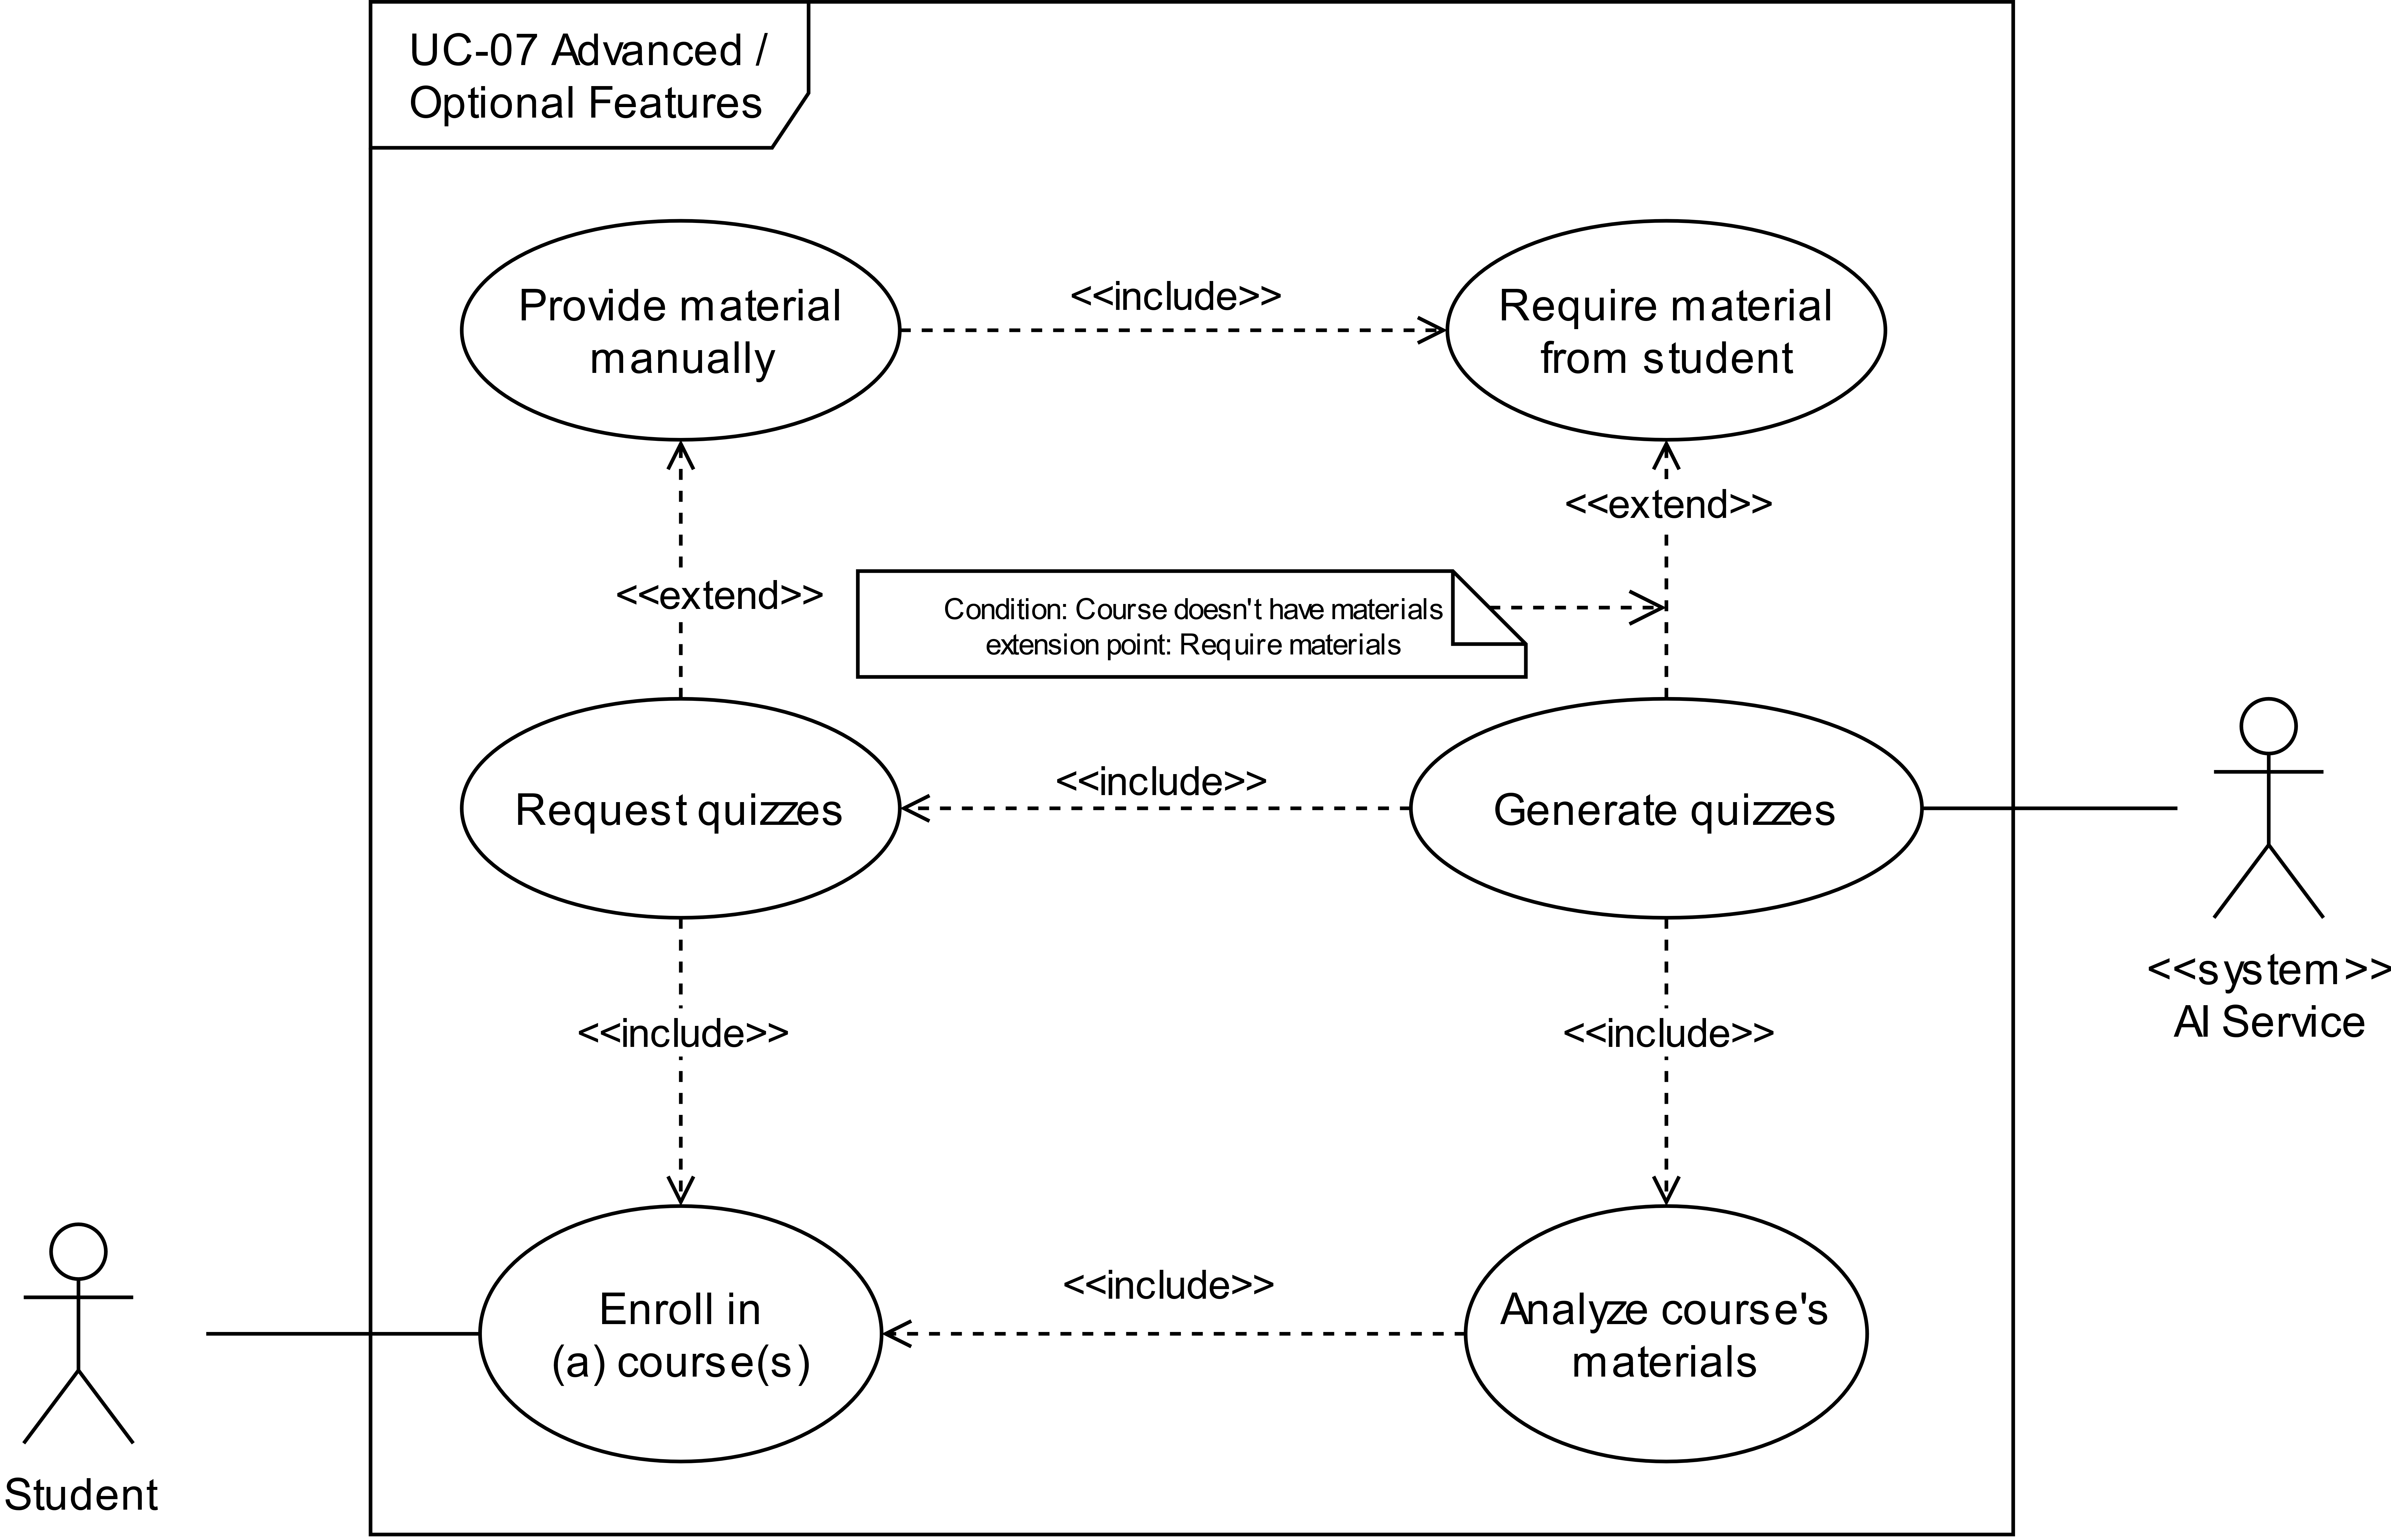
\includegraphics[width=0.9\linewidth]{images/UC-07.png}
\end{center}

\begin{center}
\textbf{Figure 8:}  AI-generated review quizzes
\end{center}

\begin{table}[h!]
\centering
\begin{tabular}{|p{3cm}|p{11cm}|}
\hline
\textbf{Use-case ID} & UC-07 \\
\hline
\textbf{Use-case name} & AI-generated review quizzes \\
\hline
\textbf{Use-case overview} & Provide students with quizzes related to the courses they are enrolling. \\
\hline
\textbf{Actors} & Students, AI service \\
\hline
\textbf{Preconditions} & 
1. The system is running. \newline
2. Internet connection is available. \newline
3. AI service must be available. \newline
4. The courses must have learning materials uploaded by tutors. \\
\hline
\textbf{Trigger} & Students use the AI-based quiz generation function. \\
\hline
\textbf{Steps} & 
1. Retrieve uploaded course materials of the course. \newline
2. Process and analyze the content with AI. \newline
3. Search the internet for related academic resources and quizzes. \newline
4. Generate quiz questions covering the key topics. \newline
5. Display the quiz to the requested students. \\
\hline
\textbf{Postconditions} & 
1. The quizzes are displayed on the screen of the requested students, and they can download the quizzes as a document file. \newline
2. The quizzes can be available until the end of the login session of the requested students, or until they finished the course if they chose to save the quizzes \\
\hline
\textbf{Alternative Flows} & 
- If the course doesn't have any learning materials, notify the user and request them for manual typing in key topics needed for review.
A1: Invalid login → Access denied with error message. \\
\hline
\textbf{Exception Flow} & 
1. If AI service isn't available, display an error. \\
\hline
\end{tabular}
\caption{Use Case UC-07: AI-generated review quizzes}
\end{table}


\newpage

